% !TEX root = main.tex
\chapter{序論}
\section{研究背景}
\subsection{半導体レーザー}
\subsubsection{半導体レーザーの現状}
半導体レーザーが実現されたのは1962年のことである 。キャリアと光の閉じ込めを能率よくできるようにした2重ヘテロ構造が用いられ流ようになり実用化・発展を遂げた。光通信、光ディスク用発光デバイスの核をなす技術である。他のレーザーにと比較しても小型・軽量、大量生産可能、熱や振動(安定性)に強い、高い発振波長選択性などが主な理由である。近年では半導体からピコ秒程度の超短光パルスを発生させる技術も研究が盛んに行われており、産業への応用が期待されている。
%[利得スイッチングsds生物発光yokoyamaさん,ここではGSにこだわらなくてもいいか][psパルスを使った産業]
\subsubsection{超短パルス発生}
ピコ秒オーダーの超短パルスを発生する技術は長距離光ファーバー伝送\cite{ref_hasegawa}に加えて、精密レーザー加工\cite{ref_chichkov} や多光子励起顕微鏡を用いたバイオイメージング[]など、応用の幅が広がってきている技術である。

半導体レーザーを用いた短パルス発生の代表的な方法としては利得スイッチングとモード同期法がある。利得スイッチング\cite{ref_h_ito}は注入電流を変調する直接変調を用いた方法である。デバイスにナノ秒程度の電流パルスを注入すると励起パルスよりも短い、数十psの光パルスが得られるというものである。半導体内の光強度が大きくなると誘導放出によって利得が急激に減少するためである。特徴としては複雑な構造を必要とせずずべての半導体レーザーで実現可能な技術であるという点である。

一方のモード同期法はサブps程度の超短パルスを得ることができる技術である。外部共振器あるいは共振器内に過飽和吸収体を挿入するなど付加的な構造が必要となる。

本研究では比較的容易に実現できる利得スイッチングに注目する。
\begin{comment}
 半導体から短パルスを発生させる方法として従来行われてきた方法が主に3つある。モード同期法、Qスイッチ法、利得スイッチ法である。モード同期法は個体レーザーでも用いられておりフーリエ限界に近いパルス幅を生成できる反面パルスの繰り返し周期が固定されてしまうという特徴を持つ。一方Qスイッチング法は過飽和吸収帯を用いるなどしてQ値を瞬間的に増大させることで高エネルギーの光パルスを得ることができる。利得スイッチングは電流を変調する直接変調の一種であり、複雑な構造を必要とせず、全ての半導体レーザーで実現が可能な技術である。レーザー加工などの技術的応用においては繰り返し可変であることや様々な種類の光源を試すことができるという利点があるため、??本研究では利得スイッチング法に着目した。
\end{comment}


\subsubsection{利得スイッチング法}
利得スイッチングは光通信技術を念頭に置いた短パルス光発生の進歩の過程で観測された。その後電源として用いるパルスジェネレーターの進歩などにより研究が進み、報告も盛んに行われてきた。図\ref{fig:fig_1_1_GS_ito}bに過去40年間に報告されてきた利得スイッチングのパルス幅がプロットされている。赤が光励起、青が電流注入を表している。電流注入の報告を見てみると最短でも5ps程度である。

また、応用としては利得スイッチングを利用した生物発光イメージの撮像の報告がある[]


次に利得スイッチングの基本的な動作について述べる。


利得スイッチング動作は半導体中のレーザー動作特性を記述するレート方程式により理解されている\cite{ref_lau}。
レート方程式はデバイス中のキャリア密度と光子密度の時間変化の振る舞いを以下のような連立方程式で表している。nは量子井戸1層あたりのキャリア密度、sは全活性層の光子密度を表す。式(\ref{eq:late_eq_1})はnの時間変化を記述している。右辺第1項は外部から注入されるポンプキャリア、第2項は誘導放出、第3項は自然放出を表す。式(\ref{eq:late_eq_2})は光子の時間変化を記述しており、第1項は誘導放出による増幅、第2項は光子寿命による減衰(共振器寿命)、第3項は自然放出光による増幅を表す。
\begin{eqnarray}
\dfrac{dn}{dt}&=&n_{\rm{pump}}\zeta(t)-\dfrac{\Gamma}{m}\nu_{\rm{g}}g(n)\dfrac{s}{1+\epsilon s}-\dfrac{n}{\tau_{r}}\\
\label{eq:late_eq_1}
\dfrac{ds}{dt}&=&\Gamma\nu_{g}g(n)\dfrac{s}{1+\epsilon s}-\dfrac{s}{\tau_{p}}+m\beta\dfrac{n}{\tau_{r}}
\label{eq:late_eq_2}
\end{eqnarray}
\begin{eqnarray*}
&n& : 量子井戸1層あたりのキャリア密度 [m^{-3}]\\
&s& : 活性層全体の光子密度[m^{-3}]\\
&n_{\rm{pump}}& : 励起キャリア密度 \\
&\zeta(t)& : 規格化された励起パルスの時間変化\\
&\Gamma & : 光閉じ込め係数\\
&m& : 量子井戸数\\
&\nu_{g}& : 群速度[m/s]=c/n_{eq}?\\
&g(n)& : 利得[cm^{-1}]\\
&\epsilon & : 利得圧縮係数?\\
&\tau_{r}& : キャリア寿命[s^{-1}]\\
&\tau_{p}& : 光子寿命 [s^{-1}]\\
&\beta& : 自然放出光係数\\
\end{eqnarray*}

上式のようなレート方程式を基に短い励起パルスを印可した時の発光および利得の時間変化についてシミュレーションを行った結果を図\ref{fig:fig_1_1_GS_ito}aに示す。赤線が光励起によるインパルス励起の様子、青線が電流注入による数ns秒パルス励起の様子である。青線に注目すると図\ref{fig:fig_1_1_GS_ito}a上段での励起パルスよりも短い、数十ps光パルスが出てくることがわかる。さらに1つ目のパルスの後は緩和振動が起きている。これが典型的な利得スイッチング動作である。また下段には利得の時間変化が示されている。励起が始まると同時に電子密度つまり利得が増えていき、ある時刻をすぎると閾値に達し反転分布を形成する。今度は誘導放出によって一気にキャリアが放出される。このキャリアの消費が注入されるキャリアよりも大きくなるため、利得も急激に減衰し、光パルスも急峻に立ち下がる。これが利得スイッチングの理解である。

\begin{figure}[h]
	\centering
	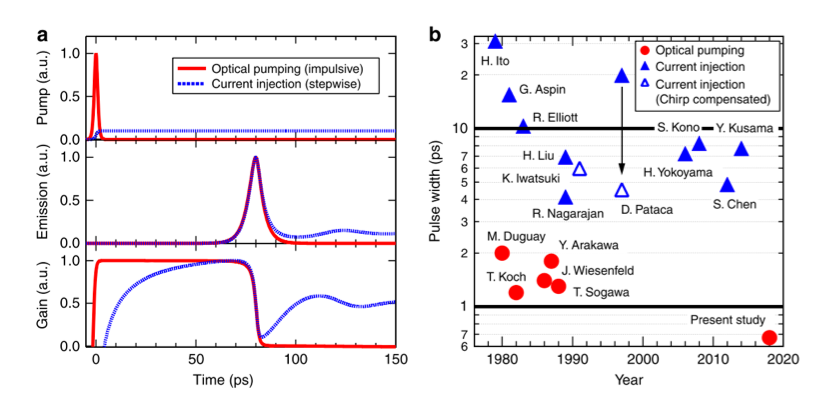
\includegraphics[width=15cm]{figure/fig_1_1_GS_ito.png}
	\caption{a 利得スイッチングのメカニズム, b過去の研究におけるパルス幅\cite{ref_t_ito}}
	\label{fig:fig_1_1_GS_ito}
\end{figure}


レート方程式の誘導放出の項に関わってくる利得$g(n)$はキャリア密度nに比例する線形利得$g_{0}(n-n_{0})$のような形で近似されてきた($g_{0}$は利得定数,$g_{0}$は透明キャリア密度)。しかしchenらはg{n}に非線形な項を取り入れたシミュレーションを行った。利得を式(\ref{eq:nonlier_gain})のように記述した。線形な項に加えて、$g_{s}$といった利得飽和の効果を取り入れている。図\ref{fig:fig_1_1_GS_pulse}にこの時のパルス生成中のキャリア密度、光子密度および利得の時間変化を表す。時刻0で2psのインパルス励起行った時の光の時間波形赤の実線と破線、キャリア密度を緑の線、材料利得を青い線で表している。
\begin{eqnarray}
g(n)&=&g_{0}(n-n_{0})\left[1+\dfrac{g_{0}(n-n_{0})}{g_{s}}\right]^{-1}\\
\label{eq:nonlier_gain}
&\simeq &\left\{
\begin{array}{ll}
 g_{0}(n-n_{0}) & n-n_{0}\ll g_{s}/g_{0}\nonumber \\
g_{s} & n-n_{0}\gg g_{s}/g_{0}\nonumber
\end{array}
\right.
\end{eqnarray}
するとIとIIの領域つまり立ち上がりの時間領域では光子密度が小さい一方でキャリア密度が大きいため、$g_{s}$が支配的に立ち上がりを決めている。IIIの領域ではキャリア密度が減少し、利得が線形になってくる領域では$\epsilon$が効いてくる。IVの領域ではキャリア密度も光子密度も小さくなっているため減衰の速さは光子の共振器寿命$\tau_{p}$によってきまる。

共振器寿命$\tau_{p}$は
\begin{eqnarray}
\tau_{p}=\dfrac{n_{eff}(1/\alpha_{a})/c}{1+(\alpha_{m}/\alpha_{a}}=\dfrac{n_{eff}/c}{\alpha_{a}+\alpha_{m}}
\end{eqnarray}
とかける\cite{ref_iga}。
$\alpha_{a}$は平均吸収損失、cは光速、$\alpha_{m}$は共振器の反射損であり、
\begin{eqnarray*}
\alpha_{m}=(1/L)ln(1/R_{m})+\alpha_{d}
\end{eqnarray*}
である。Lは共振器長、Rは共振器のミラーの反射率、$\alpha_{d}$は反射鏡が有限の大きさであるために生じる回折損失である。


多重量子井戸にすることと$g_{s}$には関係があるんだっけ?ない


このように利得スイッチングには興味深い非線形性が含まれており詳細に理解を進めることは半導体レーザーそのものの理解にも繋がりうる。

\clearpage
\subsubsection{利得スイッチング光パルスの短パルス化}


\begin{figure}[h]
	\centering
	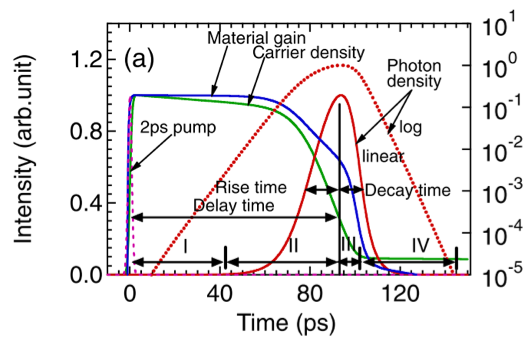
\includegraphics[width=15cm]{figure/fig_1_1_GS_pulse.png}
	\caption{パルス生成中のキャリア密度、光子密度、利得gの時間変化\cite{ref_1_1_GS}}
	\label{fig:fig_1_1_GS_pulse}
\end{figure}

\clearpage
\subsection{InGaAs高利得材料}
先の節で活性層を高利得化することによる利得スイッチングパルスの高速化が見込めることについて述べた。では実際にはどのような結晶構造にするのが高利得材料となり得るのだろうか。

本研究では量子井戸の数を増やし、多重量子井戸を形成することにより高利得化を図った。本節では量子井戸の多重化とその際に生じる結晶の歪みについて述べる。
\subsubsection{量子井戸レーザー}
まず量子井戸レーザーであるが、井戸の中の電子のエネルギーが離散値をとるので発振波長の短波長化が図れる(どうでもよくない?)
、閾値電流密度の温度変化が小さい、(バンド端の状態密度が大きいことに由来)、再結合効率が大きい(キャリアが量子井戸に閉じ込められることに由来)などの特徴を有する。


量子井戸レーザーは1975年Van der ZielらによってMBEにより始めて作られた。[]HolonyaらはMOCVD法により量子井戸レーザーの作製を行い閾値電流の温度依存性が量子井戸レーザーでは抑えられることなどを指摘した[]。その後Tsangにより$0.25kA/cm^{2}$の程閾値電流密度をもつ量子井戸レーザーが発表され注目を集めた。近年では様々な材料の量子井戸レーザーが作られている。
\subsubsection{多重量子井戸レーザー}
量子井戸レーザーの特徴の1つとして量子井戸の厚さ、数のデザインが可能である。という点があげられる。数mに注目する。単一量子井戸とm周期多重量子井戸を比較した場合、透明電流はm倍になる反面、状態密度がmに比例して大きくなることによりモード利得もm倍になることが予想される。しかしこれは利得が線形利得であることを想定した場合であい、利得の平坦化を考えると図のようにgが変化することが計算されている。[]目指す利得によって適切な井戸数を選ぶ必要があることを示唆している。


M周期多重量子井戸レーザーを単一量子井戸レーザーと比較した場合を考える。
半導体レーザーの発振条件は誘導放出の利得(光閉じ込め係数かけるモード利得)が全体の損失に等しいというものであるから、
%\begin{eqnarray}
%\Gamma g_{mod}=\alpha^{total}= \xi a_{\rm{ac}} +(1-\xi)a_{\rm{ex}}+\rm{ln}(1/R)/L
%\end{eqnarray}
\begin{eqnarray}
\Gamma g_{mod}=\alpha^{total}= \Gamma \alpha_{\rm{ac}} +(1-\Gamma)\alpha_{\rm{ex}}+(1/L)\rm{ln}(1/R)
\end{eqnarray}
と書ける。$\alpha_{\rm{ac}}$はキャリアが注入される活性層(active layer)の損失、$\alpha_{\rm{ex}}$はクラッド層の損失の平均を表す。
$L_{z}$を量子井戸の厚さ、光波の実効的な広がりの厚さを$L_{0}$とすると、$L_{z}\ll L_{0}$の場合光閉じ込め係数$\Gamma$は近似的に
\begin{equation}
\Gamma = ML_{z}/L_{0}
\label{eq:Gamma}
\end{equation}
と書ける。$L_{0}$は典型的に0.1umである。
一方注入電流については
\begin{equation}
J_{M}=MJ_{M=1}
\label{eq:J_M}
\end{equation}
という関係がある。注入電流密度はキャリア面密度Nを用いて
\begin{equation}
J_{M=1}=eN/\tau_{r}
\end{equation}
と表せる。式(\ref{eq:J_M})は多重量子井戸においては単一量子井戸と比較してM倍キャリア数まで収容が可能であり、M倍のモード利得が得られる。その反面必要な注入電流もM倍になる。(透明電流密度)もし単一量子井戸のバルク利得が注入電流と線形な関係にあるならば、つまり
\begin{eqnarray}
g=a(J_{M=1}-J_{g})
\end{eqnarray}
と書けるならば($J_{g}$は透明電流密度,aは係数)単一量子井戸レーザーの閾値電流は
\begin{eqnarray}
J^{\rm{th}}_{M=1}&=&\alpha^{total}/ \Gamma + J_{g}\nonumber\\
&=&\alpha^{total}/(aL_{z}/L_{0})+J_{g} 
\end{eqnarray}
と書ける。また多重量子井戸レーザーでは
\begin{equation}
J_{M}=\alpha^{totla}/(aL_{z}/L_{0}) + MJ_{g}
\end{equation}
となる。常に単一量子井戸レーザーの方が低い閾値電流を与えることになる。これはバルク利得が注入電流に対して線形な場合の結論である。


モード利得のずほしい


言いたいこと
要は多重にするとモード利得が大きくなるため高速化に適している。

\subsubsection{量子井戸レーザーにおける歪効果}
前節で多重量子井戸化することによる利点を述べたが多重化することによる別の効果についても歴史がある。

量子井戸レーザーをさらに高性能化する手法として用いられている歪み量子井戸レーザーについて述べる。量子井戸の活性層とバリア層の結晶格子定数に違いにより歪みが発生することを利用している。

%歪みレーザーの特徴をちょっとのべる。

一般にヘテロ結合においては格子定数が異なるために内部応力が生じる。内部に歪みを含んだまま膜を作成することができ、これを歪み超格子という。図\ref{fig:fig_lattice_strain02}に模式図を示す。ヘテロ界面に平行な井戸方向の歪みを$\epsilon_{\|}$、垂直な歪みを$\epsilon_{\bot}$とした。このとき体積変形(静水圧変形)と軸方向変形の合成を見ると
\begin{eqnarray}
\epsilon_{\rm{vol}}&=&\Delta V/V=\epsilon _{xx}+\epsilon _{yy}+\epsilon_{zz}\simeq \epsilon_{\|}\\
\epsilon_{\rm{ax}}&=&\epsilon_{\bot}-\epsilon_{\|}=-\dfrac{C_{11}+2C_{12}}{C_{11}}\epsilon_{\|}-2\epsilon_{\|}
\end{eqnarray}
と書ける。$C_{11}$と$C_{12}$は弾性スティフネスと呼ばれる値で通常正四面体結晶構造の半導体では$C_{11}\simeq 2C_{12}$の関係が成り立つ。
歪みの発生により決勝内部に応力エネルギーが蓄えられる。このエネルギーが転移の発生に必要なエネルギーを超えなければ結晶は安定となる。応力エネルギーは膜厚に比例するため転位が発生しない最大の膜厚が存在する。これを臨界膜厚と呼ぶ。
Matthewsらは多重薄膜構造において転移の発生しない限界の層厚$H_{c}$を理論的に次のように導いている。\cite{ref_Matthews}
\begin{eqnarray}
h_{c}=\dfrac{b(1-\nu \cos ^2 \alpha)}{2\pi f (1+\nu ) \cos \lambda}\left(\rm{ln}\dfrac{h_{c}}{b}+1\right)
\end{eqnarray}

ここで$b=a\sqrt{2}、f=2\epsilon、\nu : ポアソン比、\alpha : 転移線とバーガースベクトスのなす角、\lambda : すべり面と海面の光線に垂直な面の方向をすべり面の方向のなす角$である。
\begin{figure}[h]
	\centering
	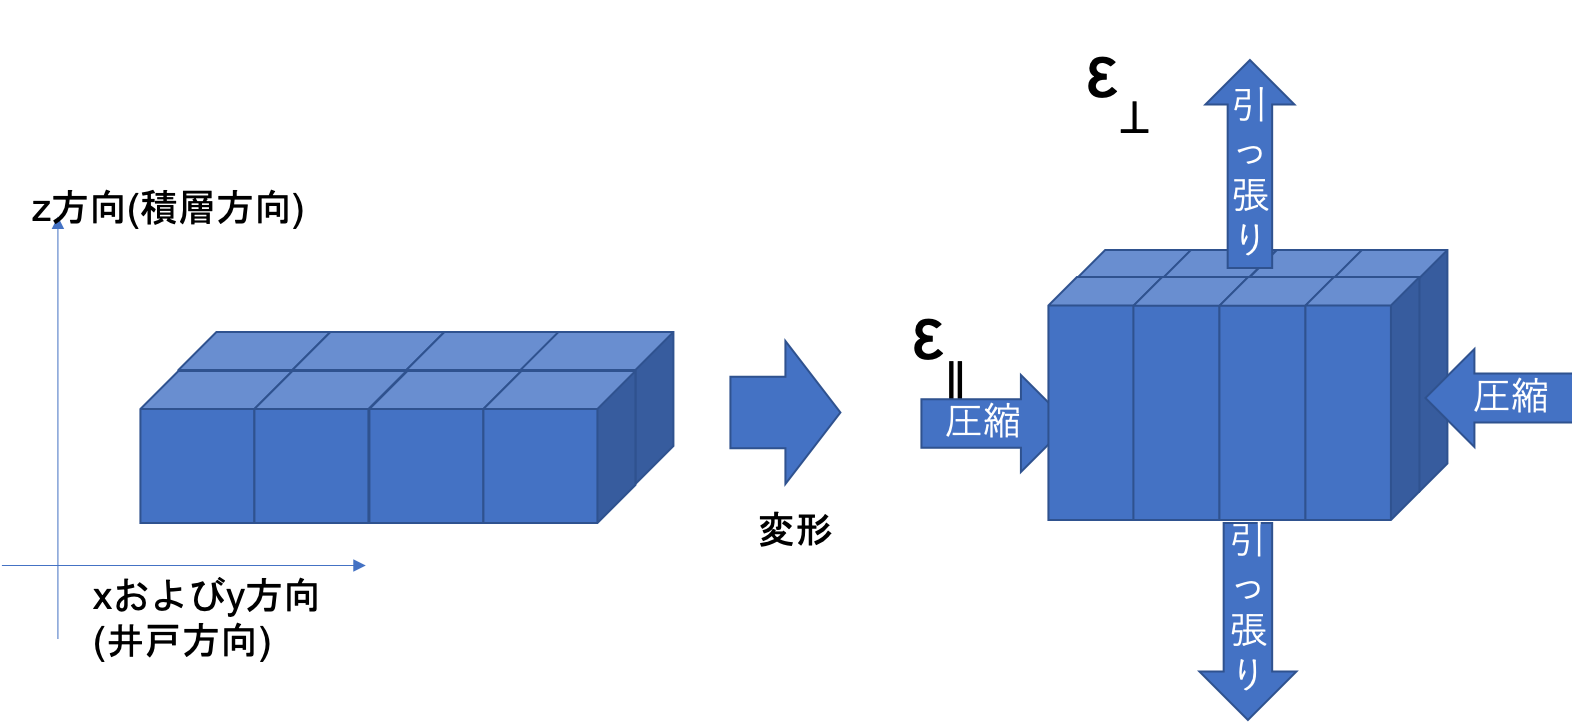
\includegraphics[width=10cm]{figure/fig_1_1_lattice_strain02.png}
	\caption{歪み模式図}
	\label{fig:fig_lattice_strain02}
\end{figure}
ここで歪みがある場合のバンド構造の変化およびそれが及ぼすレーザー特性について定性的に述べる。

体積変形歪みは伝導帯と価電子帯のバンドたんをシフトさせバンドギャップ$E_{g}$を$\Delta E_{g}=a\epsilon_{\rm{vol}}$だけ変化せさせる。aは静水圧変形ポテンシャルと呼ばれる定数である。InGaAsだと....。一方軸性変形歪みは価電子対構造を変化させ、量子井戸レーザーの特性変化の主要因となっている。歪みがない半導体では価電子帯の頂上はヘビーホールとライトホールが縮退しているが、軸性歪みにより縮退が解けてそれぞれの頂上が上下反対方向にシフトする。バンドの分離量は$E_{ll-hl}\simeq -2b\epsilon_{\rm{ax}}$で与えられる。bは軸性変形ポテンシャルと呼ばれる。


%ここに$k_{\|}$方向の図ほしい

圧縮歪みの場合、一番上の量子化準位の$k_{\|}$方向のバンド構造はライトホールになっている。すると有効質量が小さく、すなわち状態密度が小さい。するとキャリア注入による義フェルミ準位の変化が大きくなり反転分布が生じやすくなる。(反転分布の条件:$E_{fc}-E_{fv}>h\omega _{p}\geq E_{g}$を達しやすくなる)したがって発振閾値ガム歪みに比べて小さくなる。引っ張り歪みの場合準位感分離が大きくなると価電子帯混合の影響が減って$k_{\|}$方向の有効質量が小さくなる。これにより閾値を下げることが可能である。光ファイバ通信用の1.55um帯で低い閾値電流密度が報告されている。\cite{ref_thijs}xは$In_{x}Ga_{1-x}As$のx。引っ張り歪みが0,0.9,.1,1.5,2.2の単一量子井戸レーザーについて閾値電流が低くなることを報告した。

\begin{figure}[h]
	\centering
	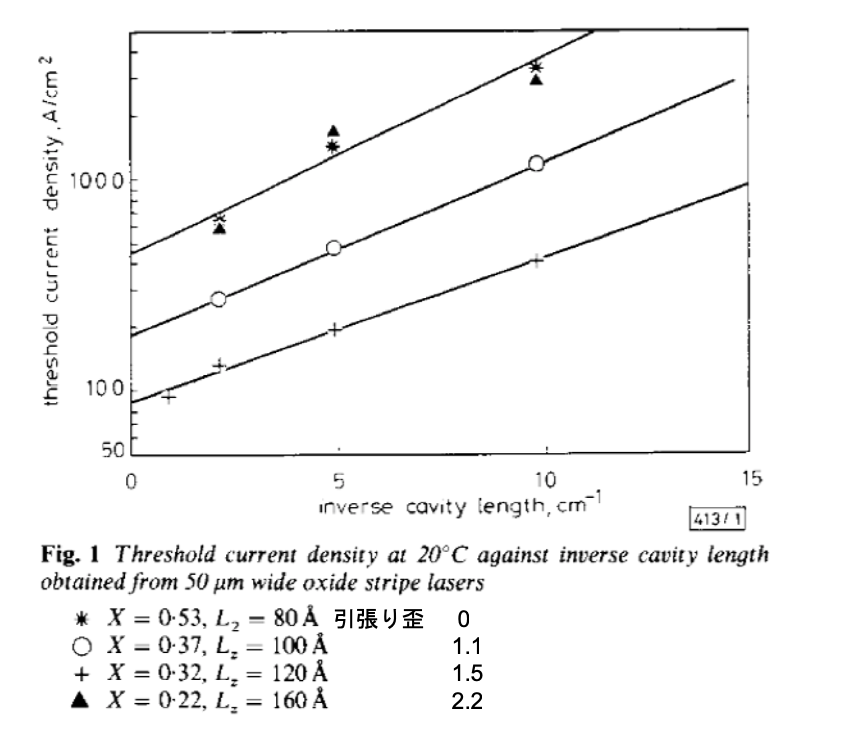
\includegraphics[width=10cm]{figure/fig_1_1_lattice_strain_Ith.png}
	\caption{単一歪み量子井戸レーザーの閾値電流密度\cite{ref_thijs}}
	\label{fig:fig_latice_strain_Ith}
\end{figure}

%じゃあ3QWの利得計算してみれば?ってなるよね
\clearpage
\subsubsection{InGaAs歪補償レーザー}
式(\ref{eq:Gamma})からわかるように多重量子化することで光閉じ込め係数を増大させ正味の利得を増やすことができる。しかし多重量子化を行うにも格子不整合による歪が生じるために活性層を積むことのできる限界の厚さが存在する。

そこで活性層の歪みをバリア層で補償する歪補償量子井戸が導入された。図\ref{fig:fig_1_1_lattice_constance}に示すように、GaAsよりも格子定数が大きなInGaAsと小さなInGaPをnmスケールで交互に結晶成長することで\rm{InGaAs}層に生じる圧縮歪をGaAs層に生じる引っ張り歪みで相殺することができる。
歪補償の条件は以下の式で表される。
\begin{eqnarray}
<a>=\dfrac{a_{well}L_{well}+a_{barrier}L_{barrier}}{L_{well}+L_{barrier}}=a_{substrate}
\end{eqnarray}
格子整合の模式図を図\ref{fig:fig_1_1_lattice_strain_comp}に示す。
歪補償により微分利得の増加の報告もある。\cite{ref_Dutta}。DuttaらはInGaAs/GaAs系3周期歪量子井戸レーザーとInGaAs/GaAsP系4周期歪補償量子井戸レーザーの線形利得をそれぞれ$dg/dn$=1.0$\times 10^{-15}\rm{cm^{2}}$、と$dn/dt$=2.1$\times 10^{-15}\rm{cm^{2}}$と見積もっている。

歴史的には歪補償を行うことにより発光スペクトルおよび吸収スペクトルのの長波長化も目的とされていた。

\begin{figure}[h]
	\centering
	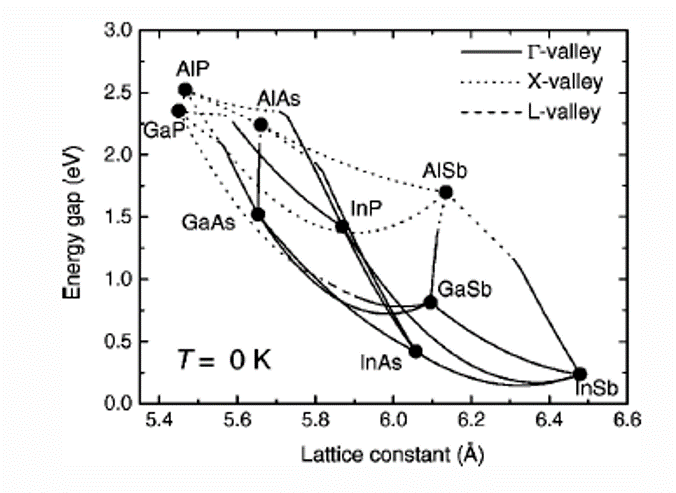
\includegraphics[width=15cm]{figure/fig_1_1_lattice_constance.png}
	\caption{格子定数}
	\label{fig:fig_1_1_latittce_constance}
\end{figure}

%歪み補償は\cite{ref_t_kawamura}
%歪み補償の説明→歪み補償を使ったレーザー→高利得のレーザー作った人いるかな
%どういう目的今まで歪補償レーザーが作られてきたのか?
%(温度特性300K以上の閾値電流の温度依存性の小さいレーザーが実現された[T.Hayakawa])余裕があったら入れる
%g_{0}が大きくなることを言cちゃダメかも
%Yb ドープファイバーで増幅可能な波長帯域
\begin{figure}[h]
	\centering
	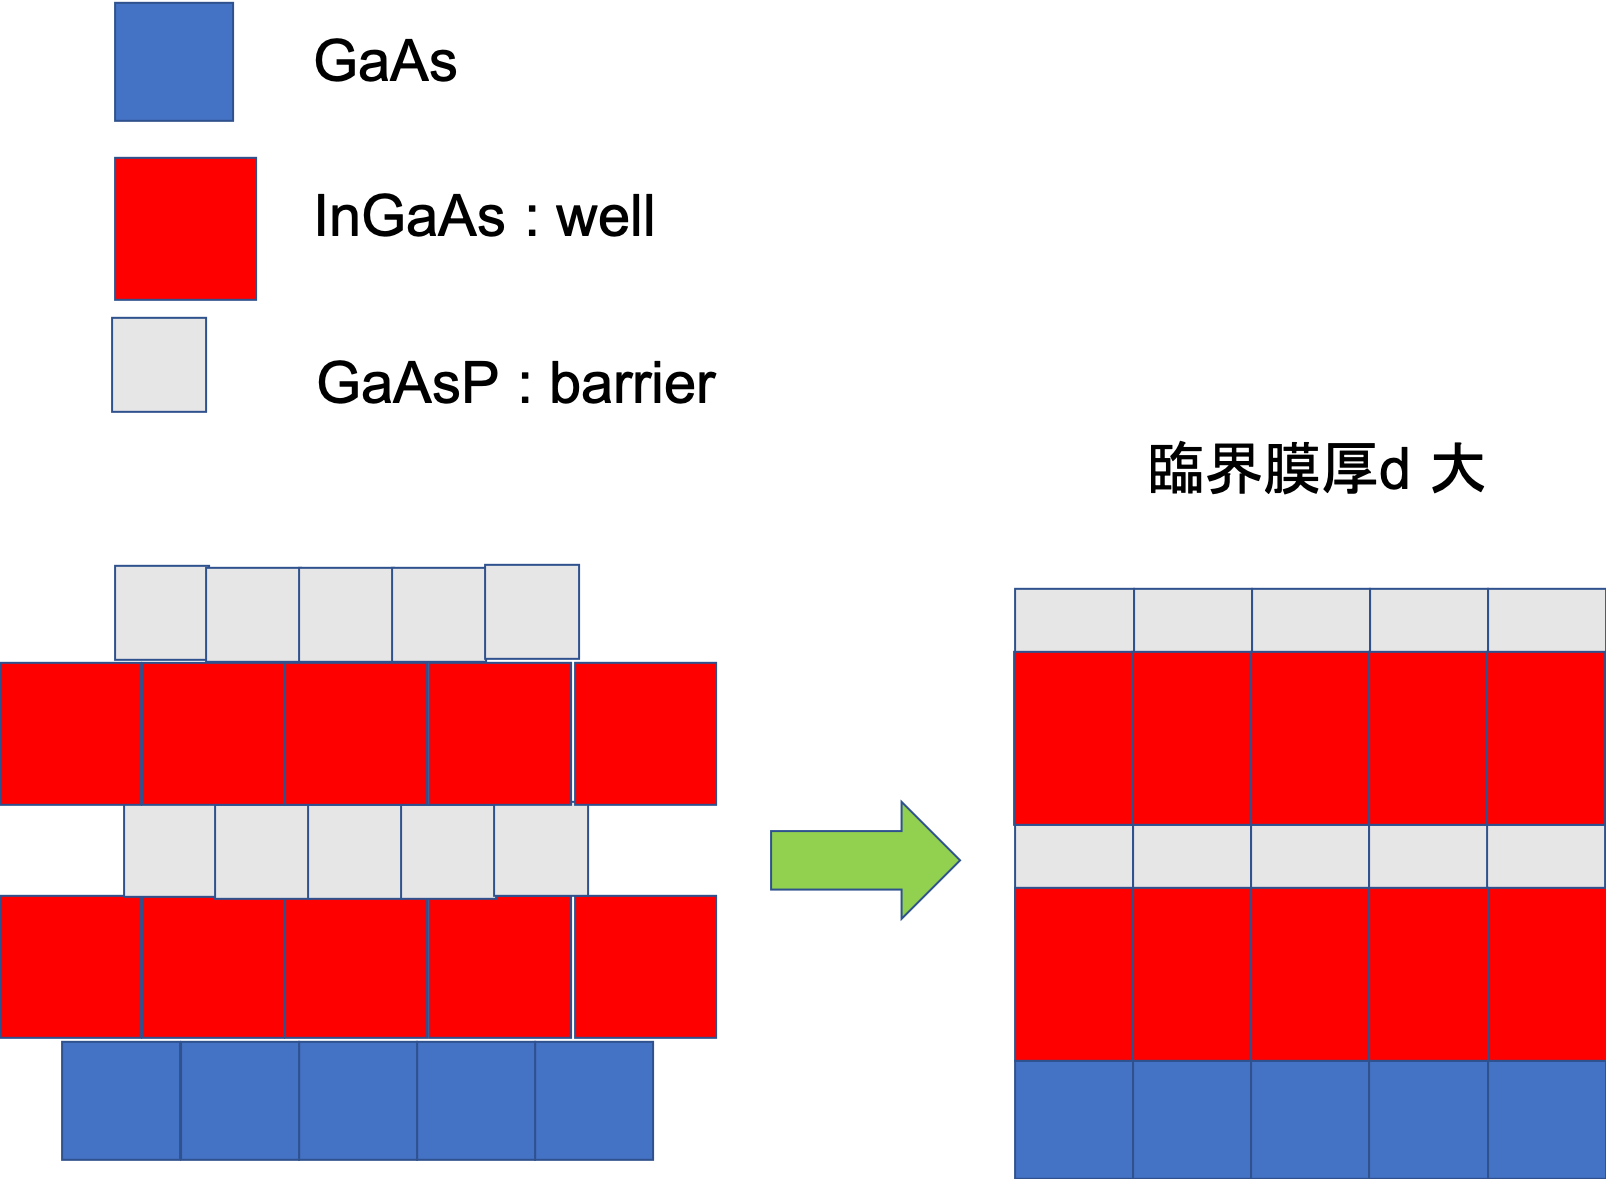
\includegraphics[width=10cm]{figure/fig_1_1_lattice_strain.png}
	\caption{歪み補償}
	\label{fig:fig_1_1_lattice_strain_comp}
\end{figure}
InGaAs

%N.K.Duttaらは歪補償4周期InGaAs/GaAsPレーザーで$\Delta g/\Delta n =2.1 \times 10^{-15}$というそれまでのレーザーよりも高い値を報告している。また。歪み補償があるものとないもので変調感度が3dB低下する周波数が似た構造のレーザーでそれぞれ32GHz、35GHzと報告している。
%もしかして10周期ってめっちゃ多い?

\clearpage
\section{本研究の目的}

従来より利得スイッチングを利用した超短パルス発生は数多く試みられてきた。半導体から直接超短パルスを発生させることの利点が非常に大きいためである。パルスを短くする工夫としてはモード利得$\Gamma g$を大きくすることが提案されてきており、そのためには量子井戸の多重化が有効である。そこで本研究では多重量子井戸化を行った高利得材料のレーザーデバイスをデザイン、作製することを目的とする。さらに作製した試料に対して電流注入実験を行い発振特性を調べ、また利得スイッチング動作を試み過去の報告に匹敵する短パルス発生が可能かを推し量ることを目的とする。